The mission of this project is to propose a Low Earth Orbit 6U sized Cubesat in order to track down the hurricanes across the South-Atlantic U.S. Region. The primary target coverage area is about 110,000 square miles across the South East-cost. This Cubesat should be able to track small to big size hurricanes across the given region. This is mainly achieved using high-tech dual cameras. It will try to collect the speed, impact area,  changes in temperature, pressure, and air composition of earth’s atmosphere for a given radius in miles. By doing so, it has to communicate and transmit data back and forth between local stations effectively. Furthermore, we must ensure the recorded data is shared with the outlined stakeholders and interested parties effectively. 
\subsection{Mission Objectives }
Our primary and secondary mission objectives are as follows.
\subsubsection{Primary  Objectives}
\begin{itemize}[noitemsep]
  \item Data recording (Wind speed, hurricane trajectory, impact radius) and analysis.
  \item Transmission of data to and from ground station up to 10 external entities.
  \item Cubesat autonomous tasking if necessary, and warning category level for immediate action.
  \item Navigation and monitoring hurricane impacted areas. Assessing damage on infrastructures to a certain degree.
  \item Updating locations using on board GPS or grounds station.
\end{itemize}
\subsubsection{Secondary Objectives }
\begin{itemize}[noitemsep]
  \item Recording relevant data (Temperature, Pressure, Humidity) for scientific study  .
  \item Maintaining communication with weather stations every $15-20m$ minutes.
  \item Guidance and Navigation of hurricane free zones.
  \item Remote sensing capabilities and effective communication with nearby satellites to avoid debris and collision course. 
\end{itemize}

\subsection{Requirements}
\subsubsection{Functional Requirements}
\begin{itemize}[noitemsep]
  \item 
  Cubesat shall coverage a minimum of 2400x1300 square km (110,00 square miles) ground area for hurricane monitoring.
 \item 
 Cubesat shall provide 2 visible spectrum images with up to 10m/pixel or lower for narrow field, and upto 100m-200m/pixel or max for a wide range of hurricane resolution.
\item
Spacecraft shall provide temperature, relative speed, & atmospheric readings of hurricane (use infrared cam).  
\item
Must able to transmit to ground station without having to rotate the spacecraft.
  \item Responsiveness: Transmitting 3 24-bit color depth images to the ground station over a single pass spanning 15 minutes.
\end{itemize}
\subsubsection{Operational Requirements}
\begin{itemize}[noitemsep]
  \item Duration: Will have a mission life of at least 15-20 years
  \item Availability: 12-hour maximum outage provided space weather conditions.
  \item Reliable: Provided no external and uncontrolled space phenomenon.
  \item Communication: Updates every 15-20 min per by pass.
  \item Data content: Images, location, relative speed, hurricane radius, impact area, atmospheric data, weather prediction and forecast.
  \end{itemize}\\
\subsubsection{Subsystem Requirements and Constraints}
After going over the mission requirements, the subsystem components are inspected and checked to see if they can meet the mission purpose.  Figure \ref{fig:ssreq} goes over all our subsystem designs and lists whether that specific component's requirement and constraint. This in return shapes our design and component selection process. \\
\FloatBarrier
\begin{figure}[hbt!]
    \centering
    \includegraphics[width=\textwidth, frame]{Images/ss_req.png}
    \caption{Subsystem Requirements and Constraints}
    \label{fig:ssreq}
\end{figure} \\

\subsection{Analysis and Trade Studies}
To ensure our project results in designing an effective and efficient cubesat, we have made a project plan to provide the best out put parameters in Figure \ref{fig:manplan}. After initial mission definition the project is closely followed by trade studies. Numerous data for previous successful missions were collected firsthand. The Japanese XI \cite{EoPortal2002} cubesat, the Freja \cite{Freja} cubesat, and the Firesat from the Space mission and design \cite{Larson1999} reference were used as a basis. Those projects solely match our functionality requirements for a 1U-12U cubesat. Figure \ref{fig:graph}(a) is the volume (density) of cubesats at various altitude. It shows 6U-sats are commonly used for a wide range of altitude. If HurriSat is to be equipped with a faster imaging cameras, and max transfer (bandwidth) frequency as shown in Figure \ref{fig:graph}(b), it will require high throughput (red-accent) power. The tradeoff is an increase in mass size as shown in Figure \ref{fig:graph}(c). The inclination distribution of cubesats is graphed in Figure \ref{fig:graph}(d) in order to provide some insight on satellite footprint with mass and altitude. 
Once we select the performance metrics, we use STK \cite{AGISolutions2021} software analysis to test the values in the simulation. After reading the feedback from the simulation; if the findings are feasible, we proceed to component design phase. If not, we go back to refine our mission definition and operational requirements. This is an agile project managing system where we select the performance parameters and perceive the coverage, operation orbit and bypass simultaneously to decide the best fit. This allows us to be flexible with the little time provided.

\tikzstyle{decision} = [diamond, fill=gray!50, text badly centered, node distance=3cm, inner sep=0pt]
\tikzstyle{block} = [rectangle, fill=red!37, text centered, rounded corners, minimum height=4em]
\tikzstyle{line} = [draw, -{Latex[width=5pt,length=7pt]}]
\tikzstyle{cloud} = [ellipse, fill=iitred, node distance=3cm, minimum height=2em]
\vspace{0.5cm}
\begin{figure}[H]
\caption{Mission Analysis}
    \centering
    \begin{tikzpicture}[node distance = 2cm, auto, text=black, inner sep=5pt, align=center]
        % Place nodes
        \node [block] (design) {Mission Definition};
        \node [block, right of = design, node distance = 3.5cm] (manufacturing) {Trade Study};
        \node [block, right of= manufacturing, node distance = 3.5cm] (assembly) {STK Analysis};
        \node [block, right of= assembly, node distance = 3.5cm] (testing) {Testing};
        \node [block, below of= assembly, node distance = 2cm] (feedback) {Feedback};
        \node [block, right of= testing, node distance = 3.5cm] (final) {CubeSat};
        
        % Draw edges
        \path [line] (design) -- (manufacturing);
        \path [line] (manufacturing) -- (assembly);
        \path [line] (assembly) -- (testing);
        \path [line] (testing) |- (feedback);
        \path [line] (feedback) -| (design);
        \path [line] (testing) -- (final);
    \end{tikzpicture}
    \label{fig:manplan}
\end{figure}
\begin{figure}[h!]
  \centering
  \subfloat[Cubesat size scatter vs altitude.]{\includegraphics[width=0.5\textwidth,scale=0.7]{Images/unit.pdf}\label{fig:unit}}
  \hfill
  \subfloat[Downlink Freq over power per unit size.]{\includegraphics[width=0.5\textwidth,scale=0.7]{Images/down.pdf}\label{fig:down}}
 \par\medskip
%   \hfill% or \hspace{5mm} or \hspace{0.3\textwidth}
  \subfloat[Power Loading]{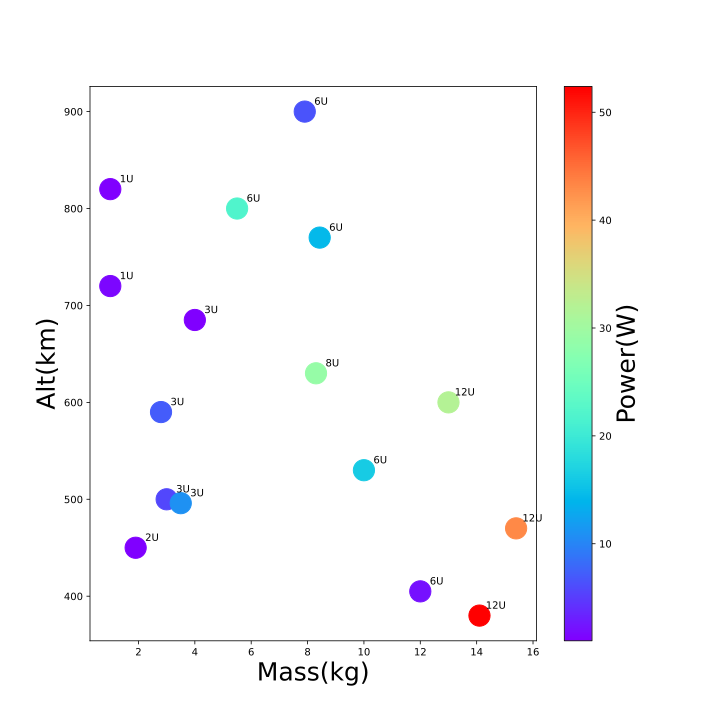
\includegraphics[width=0.5\textwidth,scale=0.9]{Images/power.pdf}\label{fig:power}}
  \hfill
  \subfloat[Inclination]{\includegraphics[width=0.5\textwidth,scale=0.9]{Images/Alpha.pdf}\label{fig:alpha}}
  \caption{Trade Studies}
  \label{fig:graph}
\end{figure}\\

\subsection {Risk Assessment}
Risk assessment assures the stakeholders whether our cubesat  is on track to be hazard free, secure, safe, and scientifically feasible. It is impossible to avoid risks completely. Thus, the team has provided a risk assessment definition in Table \ref{Tab:rd}. Those definitions are basic guideline to help assessing the risks and provide some mitigation mechanisms. They are divided in to two sections: probability and severity. Probability is the likelihood of risk to occur, while severity is the effect of the risk. To determine the risk assessments a color grading scale is provided in Table \ref{Tab:rcg}. Bright red is a high probability  and extremely severe. This risk will definitely hinder all types of operation and may even lead to complete failure of the mission. Green on the other hand is quite the opposite.\\

\begin{table}[hb!]
\centering
\caption{Risk Definitions}
\label{Tab:rd}
\begin{tabular}{ l l }
    \rowcolor{gray!50}{Risk Probability & Description}\\ \hline
    Frequent & Consistent threat to mission. Requires deliberate and active planning. \\
    Occasional& May occur a couple-three times.\\
    Improbable & Highly unlikely to occur.\\[.1in]
    \rowcolor{gray!50}{Risk Severity & Description}\\ \hline
    Catastrophic   & Would cause complete mission failure. It's a no-go situation.\\
    Major         & Would cause significant complication to mission.\\
    Minor         & Would causes a minor  hindrance to mission.\\
    Negligible    & Minimal effect on mission.        
\end{tabular}
\end{table}
\vspace{1.5cm}
\begin{table}[hbt!]
\caption{Risk Color-grading}
\label{Tab:rcg}
\centering
\resizebox{\textwidth}{!}{%
\begin{tabular}{|c|ccccc|}
\hline
                                                                                       & \multicolumn{5}{c|}{\textbf{Risk Severity}}                                                                                                                                                                            \\ \hline
                                                                                       & \multicolumn{1}{c|}{}               & \multicolumn{1}{c|}{Catastrophic (4)}           & \multicolumn{1}{c|}{Major (3)}                  & \multicolumn{1}{c|}{Minor (2)}                  & Negligible (1)             \\ \cline{2-6} 
                                                                                       & \multicolumn{1}{c|}{Frequent (A)}   & \multicolumn{1}{c|}{\cellcolor[HTML]{FE2200}A4} & \multicolumn{1}{c|}{\cellcolor[HTML]{FD6864}A3} & \multicolumn{1}{c|}{\cellcolor[HTML]{FFCC67}A2} & \cellcolor[HTML]{FFFC9E}A1 \\ \cline{2-6} 
                                                                                       & \multicolumn{1}{c|}{Occasional (B)} & \multicolumn{1}{c|}{\cellcolor[HTML]{FD6864}B4} & \multicolumn{1}{c|}{\cellcolor[HTML]{FFCC67}B3} & \multicolumn{1}{c|}{\cellcolor[HTML]{FFCC67}B2} & \cellcolor[HTML]{B0D9AF}B1 \\ \cline{2-6} 
\multirow{-4}{*}{\textbf{\begin{tabular}[c]{@{}c@{}}Risk \\ Probability\end{tabular}}} & \multicolumn{1}{c|}{Improbable (C)} & \multicolumn{1}{c|}{\cellcolor[HTML]{FFFC9E}C4} & \multicolumn{1}{c|}{\cellcolor[HTML]{FFCC67}C3} & \multicolumn{1}{c|}{\cellcolor[HTML]{B0D9AF}C2} & \cellcolor[HTML]{9AD698}C1 \\ \hline
\end{tabular}
}
\end{table}
\vspace{1cm}
Updated risk assessment are shown below. Risk assessment assures the stakeholders whether our cubesat  is on track to be hazard free, secure, safe, and scientifically feasible. It is impossible to avoid risks completely. 
Table \ref{Tab:tpr} is where we listed out every possible risk. While most of the risks are accounted for, there might still be an unforeseeable event due to sudden radiation exposure or unaccounted space debris. HurriSat will still be utilizing its propulsion driven ADCS guided by the active software tracking to avoid debris. It will also feature a double wall bumper in the structures to sustain slight damage. Similarly, some parts of the IC transistors will have to be embedded with carbon Teflon shielding to resist radiation and thermal exposure.\\


\vspace{1.5cm}
\begin{table}[ht!]
\centering
\caption{Risk Assessment}
\label{Tab:tpr}
\resizebox{\textwidth}{!}{%
\begin{tabular}{|ccll|}
\hline
\multicolumn{1}{|c|}{\textbf{Hazard}}                                                                              & \multicolumn{1}{|c|}{\textbf{Assessment}}                                                                              & \multicolumn{1}{c|}{\textbf{Risk}}                                    & \multicolumn{1}{c|}{\textbf{Mitigation}}     \\ \hline
\multicolumn{4}{|c|}{\cellcolor{gray!50}\textbf{Pre Launch}}                                                                                                                              \\ \hline
\multicolumn{1}{|c|}{Operational Cost}                                                                              & \multicolumn{1}{c|}{\cellcolor[HTML]{FFCC67}B3}                                 & \multicolumn{1}{l|}{Delayed project timeline}                        & Clear focus on fund acquisition                    
\\ \hline
\multicolumn{1}{|c|}{\begin{tabular}[c]{@{}c@{}}Environmental \\ (Dust,Humidity, Weather)\end{tabular}} & \multicolumn{1}{c|}{\cellcolor[HTML]{FFFC9E}A1}                                 & \multicolumn{1}{l|}{Hinder launch-day, minor damage to Cubesat}                         & \begin{tabular}[c]{@{}l@{}}Controlled and designated-\\ construction environment\end{tabular} \\ \hline
\multicolumn{1}{|c|}{Transportation}                                                                    & \multicolumn{1}{c|}{\cellcolor[HTML]{FFFC9E}A1}                                 & \multicolumn{1}{l|}{Damage to CubSat or team}                  & Route Planning, safe access to traffic             \\ \hline
\multicolumn{1}{|c|}{Team injury}                                                                       & \multicolumn{1}{c|}{\cellcolor[HTML]{B0D9AF}B1}                                 & \multicolumn{1}{l|}{Damage to team member and legal liability} & Safe workspace guidelines                          \\ \hline
\multicolumn{1}{|c|}{Technology Limitation}                                                             & \multicolumn{1}{c|}{\cellcolor[HTML]{B0D9AF}B1}                                 & \multicolumn{1}{l|}{Longer time and overhead}                  & Mindful design                                     \\ \hline
%%%%%%%%%%%%%
\multicolumn{4}{|c|}{\cellcolor{gray!50}\textbf{Post Launch}}                                                                                          \\ \hline
\multicolumn{1}{|c|}{\begin{tabular}[c]{@{}c@{}}Space Debris and\\  Micrometeoroids\end{tabular}} & \multicolumn{1}{c|}{\cellcolor[HTML]{FD6864}B4} & \multicolumn{1}{l|}{Fatal destruction or damage of the Cubesat}                                                             & \begin{tabular}[c]{@{}l@{}}Double Wall Bumper, Active space debris \\ tracking software\end{tabular}
\\ \hline
\multicolumn{1}{|c|}{Radiation Exposure}                                                          & \multicolumn{1}{c|}{\cellcolor[HTML]{FD6864}A3}       & \multicolumn{1}{l|}{\begin{tabular}[c]{@{}l@{}}Electronic systems, causing circuit damage \\ or system shut downs\end{tabular}} & \begin{tabular}[c]{@{}l@{}}Transistors, IC's and circuits\\ will be embedded with carbon nanotubes.\end{tabular}               
\\ \hline
\multicolumn{1}{|c|}{Thermal Damage}                                                              & \multicolumn{1}{c|}{\cellcolor[HTML]{FFCC67}A2}       & \multicolumn{1}{l|}{Electrical, mechanical component damage}                                                                    & Selecting the best Thermal resistant shield           
\\ \hline
\multicolumn{1}{|c|}{Solar Flares}                                                                & \multicolumn{1}{c|}{\cellcolor[HTML]{FFCC67}C3}       & \multicolumn{1}{l|}{Damage or destruction of CubSat}                                                                            & \begin{tabular}[c]{@{}l@{}}Active tracking of solar threats. \\ Selective Solar flare resistant design,\\ Course correction mechanisms.\end{tabular} 
  \\ \hline
\multicolumn{1}{|c|}{Foreign Satellites}                                                          & \multicolumn{1}{c|}{\cellcolor[HTML]{FFFC9E}C4}       & \multicolumn{1}{l|}{Longer time and overhead}                                                                                   & Active tracking of other Satellites                                                                                                                  \\ \hline

%%%%%%%%%%%%%%%
\multicolumn{4}{|c|}{\cellcolor{gray!50}\textbf{Launch}}                                                                                                                                                                                                                                         \\ \hline
\multicolumn{1}{|l|}{Initial Acceleration}         & \multicolumn{1}{c|}{\cellcolor[HTML]{F2C875}B2} & \multicolumn{1}{l|}{Damage due to increasing drag and friction} & \begin{tabular}[c]{@{}l@{}}Minimized induced drag, using thrusters \\ and controllers\end{tabular}           \\ \hline
\multicolumn{1}{|l|}{Mechanical Vibration} & \multicolumn{1}{c|}{\cellcolor[HTML]{F2C875}B3} & \multicolumn{1}{l|}{Structural and payload damage}              & \begin{tabular}[c]{@{}l@{}}Incorporate shock observant if possible. \\ Distribute static loads.\end{tabular} \\ \hline
\multicolumn{1}{|l|}{Acoustic Energy}      & \multicolumn{1}{c|}{\cellcolor[HTML]{F2C875}B2} & \multicolumn{1}{l|}{Structural damage}                          & \begin{tabular}[c]{@{}l@{}}Use sound suppression system and \\ pressurized leveling.\end{tabular}            \\ \hline
\end{tabular}}
\end{table}

